\documentclass[12pt, a4paper]{article}

% ── Packages ──────────────────────────────────────────────────────────────────
\usepackage[margin=2.5cm]{geometry}
\usepackage{amsmath, amssymb, amsthm}
\usepackage{tikz}
\usetikzlibrary{arrows.meta, decorations.pathmorphing, angles, quotes, calc}
\usepackage{xcolor}
\usepackage{mdframed}
\usepackage{hyperref}
\usepackage{parskip}
\usepackage{microtype}
\usepackage{enumitem}
\usepackage{booktabs}
\usepackage{caption}

% ── Colours ───────────────────────────────────────────────────────────────────
\definecolor{oceanblue}{RGB}{10, 40, 80}
\definecolor{shorecolor}{RGB}{220, 80, 60}
\definecolor{swimcolor}{RGB}{30, 160, 90}
\definecolor{sharkcolor}{RGB}{200, 50, 50}
\definecolor{orbitcolor}{RGB}{220, 170, 40}
\definecolor{boxblue}{RGB}{230, 240, 255}
\definecolor{boxborder}{RGB}{70, 100, 180}
\definecolor{resultbg}{RGB}{240, 255, 240}
\definecolor{resultborder}{RGB}{40, 140, 60}
\definecolor{warnbg}{RGB}{255, 245, 230}
\definecolor{warnborder}{RGB}{200, 120, 20}

% ── Theorem Environments ──────────────────────────────────────────────────────
\theoremstyle{definition}
\newtheorem{theorem}{Theorem}
\newtheorem{lemma}{Lemma}
\newtheorem{corollary}{Corollary}
\newtheorem{definition}{Definition}

% ── Custom Boxes ──────────────────────────────────────────────────────────────
\newmdenv[
  backgroundcolor=boxblue,
  linecolor=boxborder,
  linewidth=1.5pt,
  roundcorner=6pt,
  innertopmargin=10pt,
  innerbottommargin=10pt,
  innerleftmargin=14pt,
  innerrightmargin=14pt
]{notebox}

\newmdenv[
  backgroundcolor=resultbg,
  linecolor=resultborder,
  linewidth=2pt,
  roundcorner=6pt,
  innertopmargin=12pt,
  innerbottommargin=12pt,
  innerleftmargin=14pt,
  innerrightmargin=14pt
]{resultbox}

\newmdenv[
  backgroundcolor=warnbg,
  linecolor=warnborder,
  linewidth=1.5pt,
  roundcorner=6pt,
  innertopmargin=10pt,
  innerbottommargin=10pt,
  innerleftmargin=14pt,
  innerrightmargin=14pt
]{warnbox}

% ── Macros ────────────────────────────────────────────────────────────────────
\newcommand{\R}{\mathbb{R}}
\newcommand{\abs}[1]{\left|#1\right|}
\newcommand{\norm}[1]{\left\|#1\right\|}
\renewcommand{\vec}[1]{\mathbf{#1}}

% ─────────────────────────────────────────────────────────────────────────────
\begin{document}

% ── Title ─────────────────────────────────────────────────────────────────────
\begin{center}
  {\LARGE \textbf{The Shark \& Circle Problem}}\\[0.5em]
  {\large A Complete Mathematical Solution}\\[0.3em]
  {\small \textcolor{gray}{Classical pursuit problem — optimal escape strategy \& critical bound}}
  \vspace{0.4em}
  \hrule
\end{center}

\vspace{0.5em}

% ── 1. THE PROBLEM ────────────────────────────────────────────────────────────
\section{The Problem}

\begin{notebox}
A swimmer starts at the \textbf{exact centre} of a circular pond of radius $R$.
A shark sits on the shore and can swim along the perimeter at $k$ times the swimmer's
speed. Both move optimally. \textbf{Can the swimmer escape?}
\end{notebox}

\vspace{1em}

\begin{center}
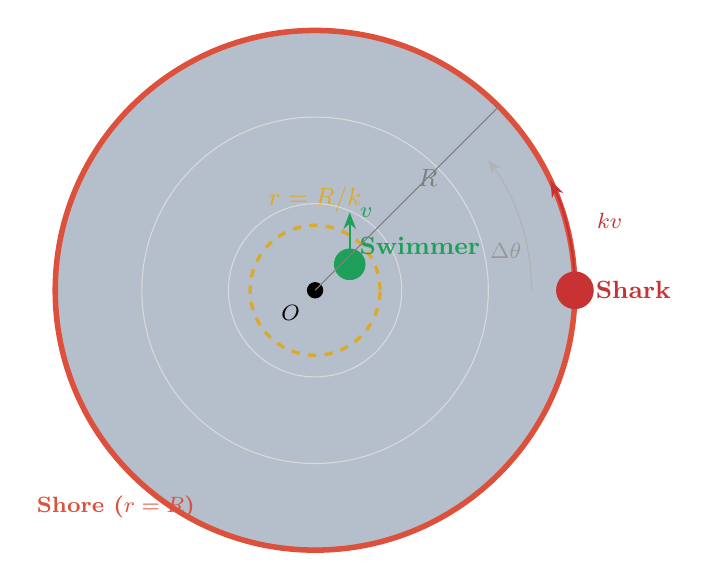
\begin{tikzpicture}[scale=1.1]
  % Ocean fill
  \fill[oceanblue!30] (0,0) circle (3cm);

  % Shore circle
  \draw[shorecolor, line width=2pt] (0,0) circle (3cm);

  % Critical orbit circle r = R/k (k = 4)
  \draw[orbitcolor, dashed, line width=1.2pt] (0,0) circle (0.75cm);
  \node[orbitcolor, font=\small\bfseries] at (0, 1.05) {$r = R/k$};

  % Range rings (subtle)
  \foreach \r in {1.0, 2.0} {
    \draw[gray!30, thin] (0,0) circle (\r cm);
  }

  % Swimmer position (inside critical circle)
  \filldraw[swimcolor] (0.4, 0.3) circle (5pt);
  \node[swimcolor, font=\small\bfseries, above right] at (0.4, 0.3) {Swimmer};

  % Swimmer velocity arrow
  \draw[-{Stealth[length=6pt]}, swimcolor, thick]
    (0.4, 0.3) -- (0.4, 0.9) node[right, font=\footnotesize] {$v$};

  % Shark on shore
  \filldraw[sharkcolor] (3, 0) circle (6pt);
  \node[sharkcolor, font=\small\bfseries, right=4pt] at (3, 0) {Shark};

  % Shark velocity arrow (CCW)
  \draw[-{Stealth[length=6pt]}, sharkcolor, thick]
    (3, 0) arc[start angle=0, end angle=25, radius=3cm];
  \node[sharkcolor, font=\footnotesize] at (3.4, 0.8) {$kv$};

  % Centre dot
  \filldraw[black] (0,0) circle (2.5pt);
  \node[font=\footnotesize, below left=2pt] at (0,0) {$O$};

  % Radius label
  \draw[gray, thin] (0,0) -- (2.12, 2.12);
  \node[gray, font=\small] at (1.3, 1.3) {$R$};

  % Angular gap arc
  \draw[-{Stealth[length=5pt]}, gray!60, thin]
    (2.5, 0) arc[start angle=0, end angle=37, radius=2.5cm];
  \node[gray!80, font=\footnotesize] at (2.2, 0.45) {$\Delta\theta$};

  % Labels
  \node[shorecolor, font=\footnotesize\bfseries] at (-2.3, -2.5) {Shore ($r = R$)};
\end{tikzpicture}
\captionof{figure}{Setup: swimmer at centre, shark on the shore, critical orbit shown dashed.}
\end{center}

% ── 2. ASSUMPTIONS ────────────────────────────────────────────────────────────
\section{Assumptions}

\begin{itemize}[leftmargin=2em, itemsep=4pt]
  \item The pond is a perfect circle of radius $R$.
  \item The swimmer starts at the origin with speed $v_s = 1$.
  \item The shark is confined to the shore and moves at speed $v_{sh} = kv_s = k$.
  \item The shark always moves to minimise the angular gap $\Delta\theta$ (optimal pursuit).
  \item The swimmer is \textbf{caught} if the shark is at the swimmer's shore landing point at the moment of arrival.
  \item Both parties have full information — they can see each other at all times.
  \item No boundaries other than the shore; no currents; continuous time.
\end{itemize}

% ── 3. KEY QUANTITIES ─────────────────────────────────────────────────────────
\section{Key Quantities}

Let the swimmer's position be $(r, \theta)$ in polar coordinates centred at $O$.
Let $\phi$ denote the shark's angular position on the shore.

\vspace{0.5em}
\begin{center}
\renewcommand{\arraystretch}{1.5}
\begin{tabular}{cll}
  \toprule
  \textbf{Symbol} & \textbf{Meaning} & \textbf{Value / Units} \\
  \midrule
  $R$             & Pond radius              & $10\,\text{m}$ (example) \\
  $v$             & Swimmer speed            & $1\,\text{m/s}$ \\
  $k$             & Shark speed ratio        & $k > 1$ \\
  $r(t)$          & Swimmer's radial distance & $r \in [0, R]$ \\
  $\theta(t)$     & Swimmer's angle          & $\theta \in [0, 2\pi)$ \\
  $\phi(t)$       & Shark's angle on shore   & $\phi \in [0, 2\pi)$ \\
  $\Delta\theta$  & Angular gap: $\theta - \phi$ & signed, wrapped to $(-\pi, \pi]$ \\
  $\omega_s$      & Swimmer's angular velocity & $\dot\theta = v\sin\alpha / r$ \\
  $\omega_{sh}$   & Shark's max angular velocity & $kv / R$ \\
  \bottomrule
\end{tabular}
\end{center}

% ── 4. THE CRITICAL RADIUS ────────────────────────────────────────────────────
\section{The Critical Radius}

\begin{lemma}[Angular Velocity Advantage]
When the swimmer is at radial distance $r < R/k$, they can orbit the centre strictly
faster than the shark can circle the shore, regardless of the direction chosen.
\end{lemma}

\begin{proof}
The swimmer's maximum angular velocity at radius $r$ is:
\[
  \omega_s^{\max} = \frac{v}{r}
\]
The shark's angular velocity on the shore is bounded by:
\[
  \omega_{sh}^{\max} = \frac{kv}{R}
\]
For the swimmer to orbit faster:
\[
  \frac{v}{r} > \frac{kv}{R}
  \quad\Longleftrightarrow\quad
  r < \frac{R}{k}
\]
Inside this radius, $\omega_s > \omega_{sh}$, so the swimmer can maintain any desired
angular gap, including widening it to $\pi$ (diametrically opposite to the shark). \qed
\end{proof}

\begin{center}
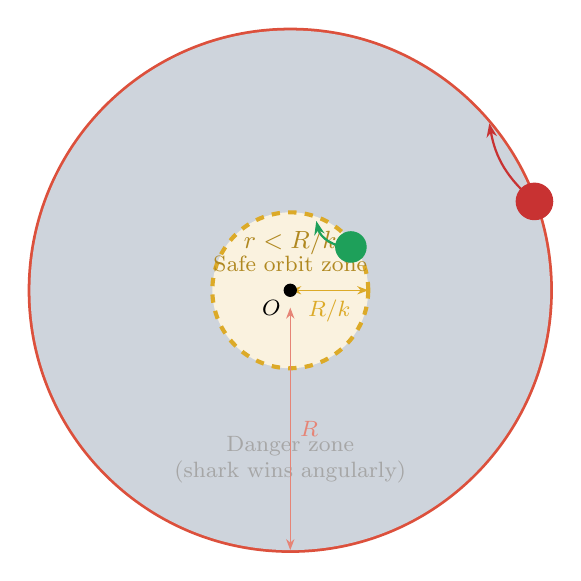
\begin{tikzpicture}[scale=1.1]
  % Shore
  \draw[shorecolor, line width=2pt] (0,0) circle (3cm);
  \fill[oceanblue!20] (0,0) circle (3cm);

  % Critical circle filled lightly
  \fill[orbitcolor!15] (0,0) circle (0.9cm);
  \draw[orbitcolor, dashed, line width=1.5pt] (0,0) circle (0.9cm);

  % Label regions
  \node[orbitcolor!80!black, font=\small\bfseries] at (0, 0.55) {$r < R/k$};
  \node[orbitcolor!80!black, font=\footnotesize] at (0, 0.3) {Safe orbit zone};
  \node[gray!70, font=\footnotesize] at (0, -1.8) {Danger zone};
  \node[gray!70, font=\footnotesize] at (0, -2.1) {(shark wins angularly)};

  % Swimmer orbiting inside
  \filldraw[swimcolor] (0.7, 0.5) circle (5pt);
  \draw[-{Stealth[length=5pt]}, swimcolor, thick, bend left=40]
    (0.7, 0.5) to (0.3, 0.8);

  % Shark on shore
  \filldraw[sharkcolor] ({3*cos(20)}, {3*sin(20)}) circle (6pt);
  \draw[-{Stealth[length=5pt]}, sharkcolor, thick, bend left=20]
    ({3*cos(20)}, {3*sin(20)}) to ({3*cos(40)}, {3*sin(40)});

  % Radius R/k annotation
  \draw[{Stealth[length=4pt]}-{Stealth[length=4pt]}, orbitcolor, thin]
    (0,0) -- (0.9,0) node[midway, below, font=\footnotesize] {$R/k$};

  % Radius R annotation
  \draw[{Stealth[length=4pt]}-{Stealth[length=4pt]}, shorecolor!70, thin]
    (0,-0.2) -- (0,-3) node[midway, right, font=\footnotesize] {$R$};

  \filldraw[black] (0,0) circle (2pt) node[below left, font=\footnotesize]{$O$};
\end{tikzpicture}
\captionof{figure}{The critical radius $R/k$. Inside it, the swimmer orbits faster than the shark.}
\end{center}

% ── 5. THE OPTIMAL STRATEGY ───────────────────────────────────────────────────
\section{The Optimal Two-Phase Strategy}

\subsection*{Phase 1 — Orbit to Gain Angular Lead}

The swimmer moves to just inside the critical radius $r^* = R/k - \varepsilon$, then orbits in the direction that \emph{increases} $\abs{\Delta\theta}$. Because $\omega_s > \omega_{sh}$ at this radius, the angular gap grows monotonically. The swimmer continues orbiting until:
\[
  \abs{\Delta\theta} = \pi
  \quad\text{(shark is diametrically opposite)}
\]

The angular rate of gain is:
\[
  \dot{(\Delta\theta)} = \omega_s - \omega_{sh} = \frac{v}{r^*} - \frac{kv}{R}
\]

Time to reach $\Delta\theta = \pi$ from zero:
\[
  T_1 = \frac{\pi}{\dfrac{v}{r^*} - \dfrac{kv}{R}}
  = \frac{\pi R r^*}{v(R - kr^*)}
\]

\subsection*{Phase 2 — Radial Sprint to Shore}

Once $\abs{\Delta\theta} = \pi$, the swimmer sprints \textbf{radially outward} toward the nearest shore point. The swimmer has angular head-start $\pi$ on the shark.

\medskip
\noindent Time to reach shore from $r^*$:
\[
  T_2 = \frac{R - r^*}{v}
\]

\noindent In this time, the shark traverses an arc of angle:
\[
  \Delta\phi = \frac{kv}{R} \cdot T_2 = \frac{k(R - r^*)}{R}
\]

\noindent The swimmer arrives at angle $\theta_0$; the shark arrives at $\theta_0 + \pi - \Delta\phi$ (measuring from the landing point). The \textbf{escape margin} in radians is:
\[
  \boxed{
    \delta_{\text{margin}} = \pi - \Delta\phi = \pi - \frac{k(R - r^*)}{R}
  }
\]

\begin{center}
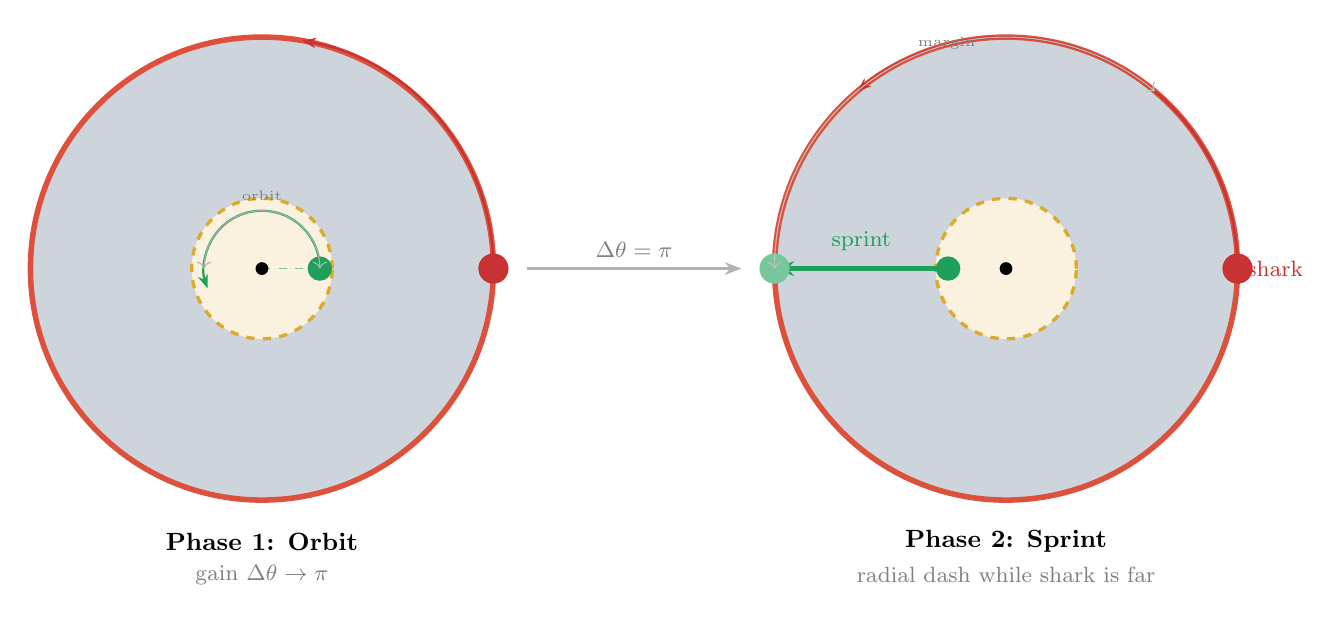
\begin{tikzpicture}[scale=1.05]
  % --- Phase 1 diagram ---
  \begin{scope}[xshift=-4.5cm]
    \fill[oceanblue!20] (0,0) circle (2.8cm);
    \draw[shorecolor, line width=2pt] (0,0) circle (2.8cm);
    \fill[orbitcolor!15] (0,0) circle (0.85cm);
    \draw[orbitcolor, dashed, line width=1.2pt] (0,0) circle (0.85cm);

    % Swimmer path (spiral inward then orbit)
    \draw[swimcolor!60, thin, dashed] (0,0) -- (0.7,0);
    \draw[swimcolor, thick, -{Stealth[length=5pt]}]
      (0.7,0) arc[start angle=0, end angle=200, radius=0.7cm];

    % Swimmer at start of orbit
    \filldraw[swimcolor] (0.7, 0) circle (4pt);

    % Shark chasing (partial arc)
    \filldraw[sharkcolor] (2.8, 0) circle (5pt);
    \draw[sharkcolor, thick, -{Stealth[length=5pt]}]
      (2.8, 0) arc[start angle=0, end angle=80, radius=2.8cm];

    % 180° gap arrow
    \draw[gray!60, thin, <->]
      (0.7, 0) arc[start angle=0, end angle=180, radius=0.7cm]
      node[midway, above, font=\tiny, gray]{orbit};

    \filldraw[black](0,0) circle(2pt);
    \node[font=\small\bfseries] at (0, -3.3) {Phase 1: Orbit};
    \node[font=\footnotesize, gray] at (0,-3.7) {gain $\Delta\theta \to \pi$};
  \end{scope}

  % --- Phase 2 diagram ---
  \begin{scope}[xshift=4.5cm]
    \fill[oceanblue!20] (0,0) circle (2.8cm);
    \draw[shorecolor, line width=2pt] (0,0) circle (2.8cm);
    \fill[orbitcolor!15] (0,0) circle (0.85cm);
    \draw[orbitcolor, dashed, line width=1.2pt] (0,0) circle (0.85cm);

    % Sprint arrow (swimmer going right)
    \draw[swimcolor, ultra thick, -{Stealth[length=7pt]}]
      (-0.7, 0) -- (-2.8, 0);
    \filldraw[swimcolor] (-0.7, 0) circle (4pt);
    \filldraw[swimcolor!60] (-2.8, 0) circle (5pt);
    \node[swimcolor, font=\footnotesize, above] at (-1.75, 0.1) {sprint};

    % Shark at opposite side (0.7, 0) then chasing
    \filldraw[sharkcolor] (2.8, 0) circle (5pt) node[right, font=\footnotesize]{shark};
    \draw[sharkcolor, thick, -{Stealth[length=5pt]}]
      (2.8, 0) arc[start angle=0, end angle=130, radius=2.8cm];

    % Gap arc
    \draw[gray!50, <->, thin]
      (-2.8, 0) arc[start angle=180, end angle=50, radius=2.8cm]
      node[midway, above right, font=\tiny, gray]{margin};

    \filldraw[black](0,0) circle(2pt);
    \node[font=\small\bfseries] at (0, -3.3) {Phase 2: Sprint};
    \node[font=\footnotesize, gray] at (0,-3.7) {radial dash while shark is far};
  \end{scope}

  % Arrow between
  \draw[gray!60, -{Stealth[length=6pt]}, very thick] (-1.3, 0) -- (1.3, 0)
    node[midway, above, font=\footnotesize, gray]{$\Delta\theta = \pi$};
\end{tikzpicture}
\captionof{figure}{Left: Phase 1 — orbit inside $R/k$ to reach a $180°$ lead.
Right: Phase 2 — sprint radially while the shark is opposite.}
\end{center}

% ── 6. THE CRITICAL BOUND ─────────────────────────────────────────────────────
\section{The Critical Bound}

For escape to be possible, the margin must be positive:
\[
  \delta_{\text{margin}} > 0
  \quad\Longrightarrow\quad
  \pi - \frac{k(R - r^*)}{R} > 0
  \quad\Longrightarrow\quad
  k < \frac{\pi R}{R - r^*}
\]

Taking $r^* \to 0$ (swimmer starts sprinting from just inside the critical circle and we optimise):
\[
  \lim_{r^* \to 0^+} \frac{\pi R}{R - r^*} = \pi
\]

But wait — if we use the optimal $r^* = R/k - \varepsilon$, substituting:
\[
  \delta_{\text{margin}} = \pi - \frac{k\!\left(R - \tfrac{R}{k}\right)}{R}
  = \pi - \frac{k \cdot R(1 - \tfrac{1}{k})}{R}
  = \pi - (k - 1)
\]

Escape requires $\delta_{\text{margin}} > 0$:
\[
  \pi - (k-1) > 0
  \quad\Longrightarrow\quad
  k < \pi + 1
\]

\begin{resultbox}
\begin{theorem}[Critical Speed Ratio]
The swimmer can escape if and only if:
\[
  k < \pi + 1 \approx 4.1416
\]
When $k = \pi + 1$, escape is exactly marginal (zero-margin). When $k > \pi + 1$, no strategy guarantees escape.
\end{theorem}
\end{resultbox}

% ── 7. ESCAPE MARGIN ──────────────────────────────────────────────────────────
\section{Escape Margin in Metres}

At the optimal sprint radius $r^* = R/k$, substituting into the margin formula:
\[
  \delta_{\text{margin}} = \pi - (k - 1) \quad [\text{radians}]
\]
Converting to \textbf{arc length} (distance along shore between swimmer and shark at landing):
\[
  \boxed{
    d_{\text{escape}} = R \cdot \bigl[\pi - (k-1)\bigr] \quad [\text{metres}]
  }
\]

\begin{center}
\renewcommand{\arraystretch}{1.4}
\begin{tabular}{cccc}
  \toprule
  $k$ & $\pi - (k-1)$ (rad) & $d_{\text{escape}}$ for $R=10$m & Escapes? \\
  \midrule
  $3.00$ & $1.14$ rad & $11.4\,\text{m}$ & \textcolor{swimcolor}{\textbf{Yes}} \\
  $3.60$ & $0.54$ rad & $5.4\,\text{m}$  & \textcolor{swimcolor}{\textbf{Yes}} \\
  $4.00$ & $0.14$ rad & $1.4\,\text{m}$  & \textcolor{swimcolor}{\textbf{Yes}} \\
  $4.14$ & $0.00$ rad & $0.0\,\text{m}$  & \textcolor{orbitcolor}{\textbf{Marginal}} \\
  $4.25$ & $-0.11$ rad & $-1.1\,\text{m}$ & \textcolor{sharkcolor}{\textbf{No}} \\
  \bottomrule
\end{tabular}
\captionof{table}{Theoretical escape margin at various shark speeds, $R = 10$ m.}
\end{center}

\vspace{0.5em}

% ── 8. THE ANGULAR GAP CONDITION ──────────────────────────────────────────────
\section{Formal Escape Condition}

Let $\phi_{\text{land}}$ be the swimmer's shore landing angle and $\phi_{\text{shark}}$ be the shark's angle at that moment. Define the capture threshold $\delta_c$ (angular half-width of the shark's reach).

The swimmer escapes if and only if:
\[
  \abs{\phi_{\text{land}} - \phi_{\text{shark}}} > \delta_c
  \quad\pmod{2\pi}
\]

In the two-phase strategy, this becomes the condition:
\[
  \pi - (k-1) > \delta_c
  \quad\Longrightarrow\quad
  k < \pi + 1 - \delta_c
\]
For any finite capture threshold $\delta_c > 0$, the bound is slightly stricter than $\pi + 1$.

% ── 9. WHY NO BETTER STRATEGY EXISTS ─────────────────────────────────────────
\section{Why No Better Strategy Exists for $k \geq \pi + 1$}

\begin{warnbox}
\textbf{Upper bound argument.} When $k \geq \pi + 1$, the shark can always cover any shore point from any other in the time the swimmer needs to travel from anywhere inside the pond to the shore.
\end{warnbox}

Formally, the swimmer must travel at least distance $R - \varepsilon$ radially (they start at the centre). The fastest this can be done is time $T_{\min} = (R - \varepsilon)/v$. In that time the shark covers arc:
\[
  kv \cdot T_{\min} = k(R - \varepsilon)
\]
For the shark to cover a full semicircle $\pi R$ (enough to reach any shore point from any starting position):
\[
  k(R - \varepsilon) \geq \pi R
  \quad\Longrightarrow\quad
  k \geq \frac{\pi R}{R - \varepsilon} \to \pi + 1 \quad \text{as} \quad \varepsilon \to 0
\]

When $k \geq \pi + 1$, the shark can always intercept — it covers more than a semicircle while the swimmer crosses from the centre region to the shore.

% ── 10. SUMMARY ───────────────────────────────────────────────────────────────
\section{Summary}

\begin{resultbox}
\textbf{The Shark \& Circle — Solution in three lines:}

\medskip
\begin{enumerate}[leftmargin=1.5em, itemsep=6pt]
  \item Stay inside $r < R/k$ and orbit to gain a $180°$ angular lead on the shark.
  \item Once opposite, sprint radially to the shore in time $T_2 = (R - R/k)/v$.
  \item Escape margin: $d = R[\pi - (k-1)]$ metres. \textbf{Escape is possible iff $k < \pi + 1 \approx 4.14$.}
\end{enumerate}
\end{resultbox}

\vspace{1em}
\begin{center}
  \small\textcolor{gray}{
    This document accompanies the browser simulation at
    \href{https://gouthamchoudary.github.io/shark_and_circle/}%
         {gouthamchoudary.github.io/shark\_and\_circle}
  }
\end{center}

\end{document}
